%
% Diseño de programa tokenizador, capítulo de análisis y diseño.
% Proyecto Lovelace.
%

\subsection{Diseño de programa tokenizador}

En la sección anterior se enlistan los algoritmos tokenizadores que
implementaremos. En esta se argumentan algunas de las decisiones tomadas
con respecto a las tecnologías usadas y se usa el \gls{gl:uml} para
describir los aspectos más significativos del programa.

\subsubsection{Vista estática del programa}

En el diagrama de la figura \ref{clases_general} se muestra una vista estática
general del programa. Las clases se dividen en dos paquetes: implementaciones
y utilidades. Las utilidades abarcan estructuras de datos, interfaces,
clases de excepciones y clases de prueba; todas ellas no tienen que ver
de forma directa con criptografía, sino que se trata de código de soporte
para las implementaciones. En las implementaciones van no solamente
los algoritmos presentados en la sección \ref{sec:algoritmos}, sino que todas
las demás clases (generalizaciones, utilidades, implementaciones de
soporte) que están relacionadas con los algoritmos tokenizadores; en el caso
de este paquete, sí todo está relacionado o con criptografía o con un
entorno bancario.

Retornando al diagrama de \ref{clases_general}: muestra solamente las clases
e interfaces directamente relacionadas con los algoritmos tokenizadores;
en las próximas secciones se mostrarán algunas otras vistas. Las utilidades
contienen las interfaces para definir los distintos tipos de funciones y la
estructura de datos (Arreglo) que se usa de manera constante en todo el
programa. Las implementaciones muestran las interfaces que definen y clasifican
a los algoritmos tokenizadores; también se muestra (por razones de espacio,
solo el nombre) las clases concretas de los sistemas tokenizadores.

Las interfaces de las funciones utilizan plantillas para definir las propias
firmas de los métodos abstractos que declaran. Esta es una forma bastante
efectiva para hacer diseños débilmente acoplados (ver
\gls{gl:acomplamiento}): por ejemplo, las redes Fesitel necesitan
de una función de ronda sobre la que \textit{no necesitan} saber nada en
particular, solo necesitan saber que la clase define un método \textbf{operar},
que es con lo que funciona el algoritmo definido por la red.

El Arreglo es una implementacion propia de una estuctura de datos de
almacenamiento secuencial. Es solamente una interfaz a una sección
de memoria (un arreglo tradicional); sin embargo, lo importante de este es
que imita el formato de las estructuras de la librería estándar de C++
(esquema de constructores y destructores para gestión de memoria, uso
de plantillas para programación genérica, etcétera). El arreglo de dígitos es
una especialización que mantiene una representación interna tanto en cadena como
en número; este arreglo es el que ocupan para comunicarse todos los
algoritmos tokenizadores. Por esta última razón es por la que se
mantienen las dos representaciones internas: algunos métodos requieren
interpretar las entradas como números y otros como cadenas.

Los algoritmos tokenizadores implementan la interfaz definida por las
funciones con inverso definiendo el tipo de ida y de vuelta como un
arreglo de dígitos (\gls{gl:pan} y \gls{gl:token}). Las interfaces intermedias
(algoritmos reversibles e irreversibles) permiten definir un comportamiento
genérico para cada tipo de algoritmo; estas a su vez declaran los métodos
abstractos que los algoritmos concretos deben de implementar.

\begin{figure}
  \begin{center}
    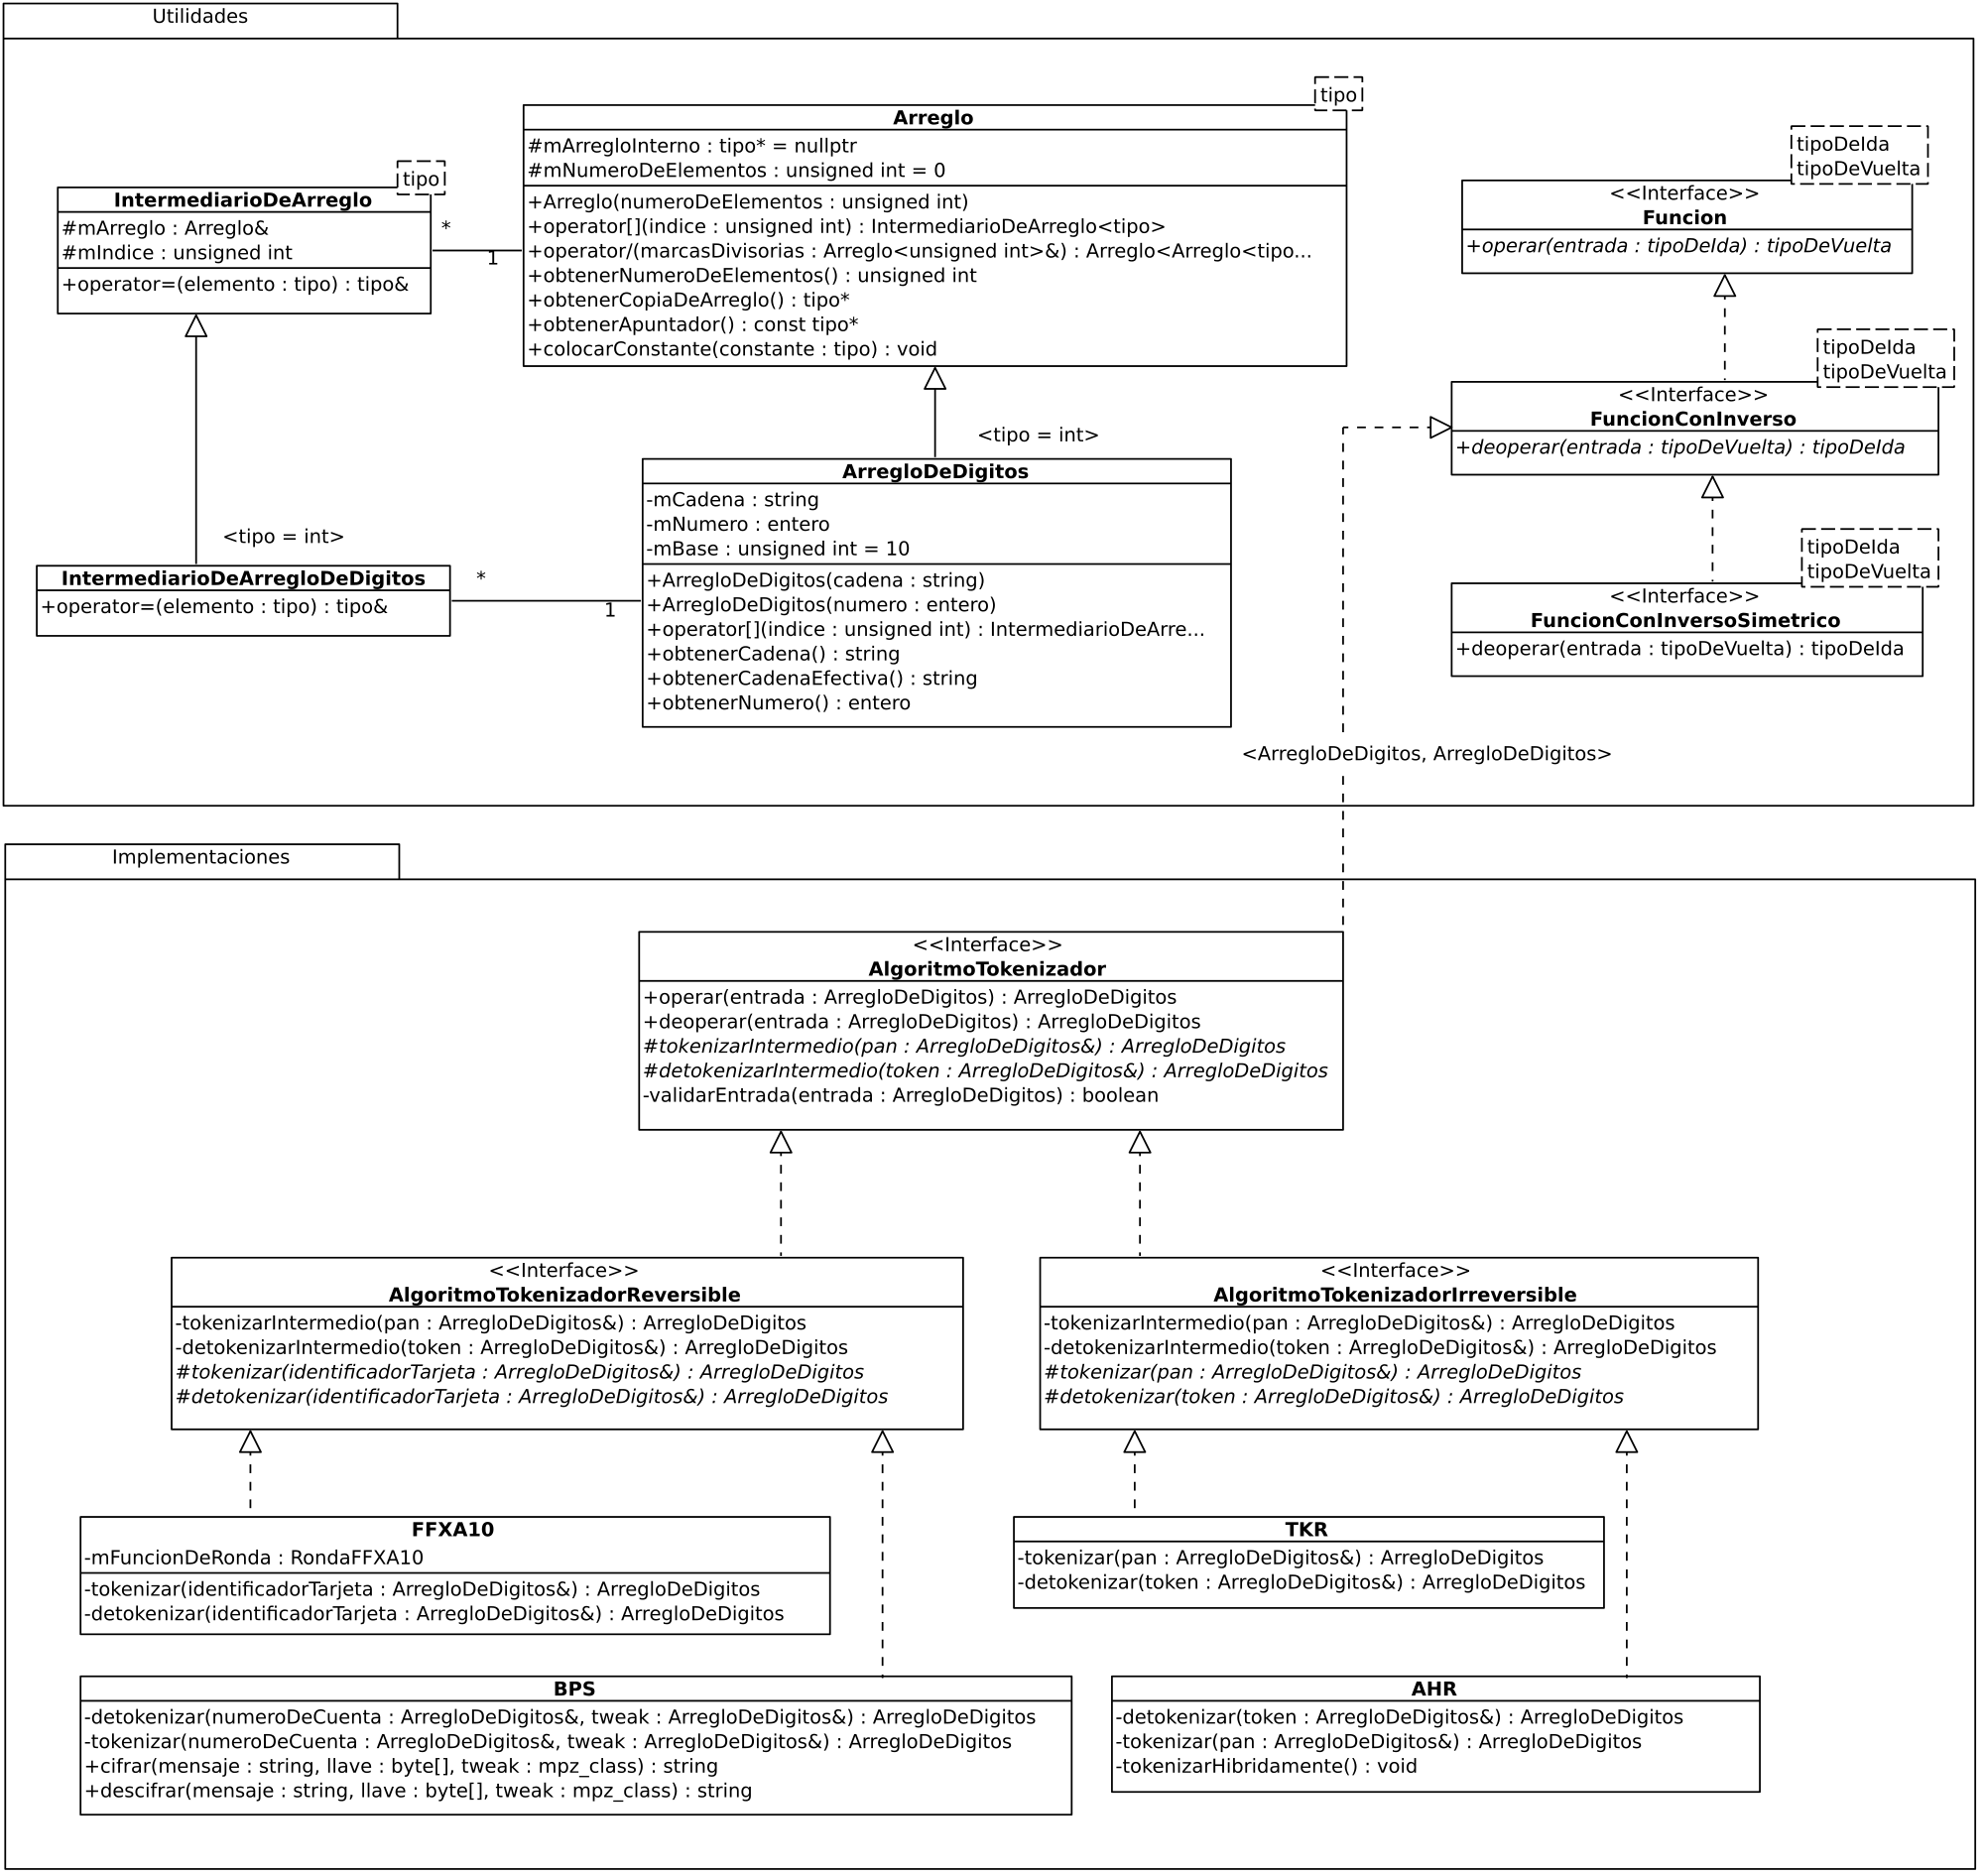
\includegraphics[width=1.0\linewidth]{diagramas/diagrama_general.png}
    \caption{Diagrama de clases general.}
    \label{clases_general}
  \end{center}
\end{figure}

\paragraph{Clases de FFX}

En la figura \ref{clases_ffx} se muestran las clases que conforman al módulo de
FFX. Sin contar a las tres interfaces de funciones (que forman parte del paquete
de utilidades) todas las clases son del paquete de implementaciones.

La clase de la red Feistel implementa la interfaz de una función con inverso
(tiene tanto operación de ida, como de vuelta) y se compone (por medio de una
relación de composición) de una función, utilizada como fucnión de ronda, y de
una función con inverso, utilizada como operador de combinación. Ambas clases
hijas (redes Feistel alternantes o desbalanceadas) contienen un indicador de
desbalanceo y sobreescriben ambas operaciones de la superclase; la red feistel
alternante (ver sección \ref{sec:red_feistel}) agrega una nueva función
de ronda: una para las pares y otra para las impares.

En la parte superior de diagrama se muestran las dos posibles operaciones de
combinación que soporta ffx: una a nivel de bloque y la otra nivel de caracter.
La única clase en donde estas dos opciones son reestrictivas es desde la
construcción de FFXA10; el desacoplamiento dado por las interfaces permite que
lo único que necesite saber la red es que tiene una función que recibe un
arreglo y entrega un arreglo.

Otra clase con la misma esructura que las dos anteriores es la de la función de
ronda de FFXA10: implementa la interfaz de una función con inverso simétrico
(que a su vez implementa un función con inverso); una instancia de esta clase
en FFX es usada para construir a la red Feistel con la que se opera.

La clase de FFX es solamente un medio de comunicación con la red Feistel
interna, esto es, no agrega ninguna lógica extra a los procesos de operación y
operación inversa. Lo mismo ocurre con FFXA10; solo que mientras el contructor
de la superclase es abierto a personalizar la red (FFX debería servir para
cualquier cifrado que preserva el formato, no solo para un alfabeto de
dígitos), el contructor de FFXA10 tiene parámetros bastante limitados, y su
construcción de la superclase y la red Feistel ya es predefinida según la
descripción de esta colección hecha en la sección \ref{sec:ffx}. Es esta última
clase (FFXA10) la que implementa la interfaz de los algoritmos tokenizadores
reversibles.

\begin{sidewaysfigure}
  \begin{center}
    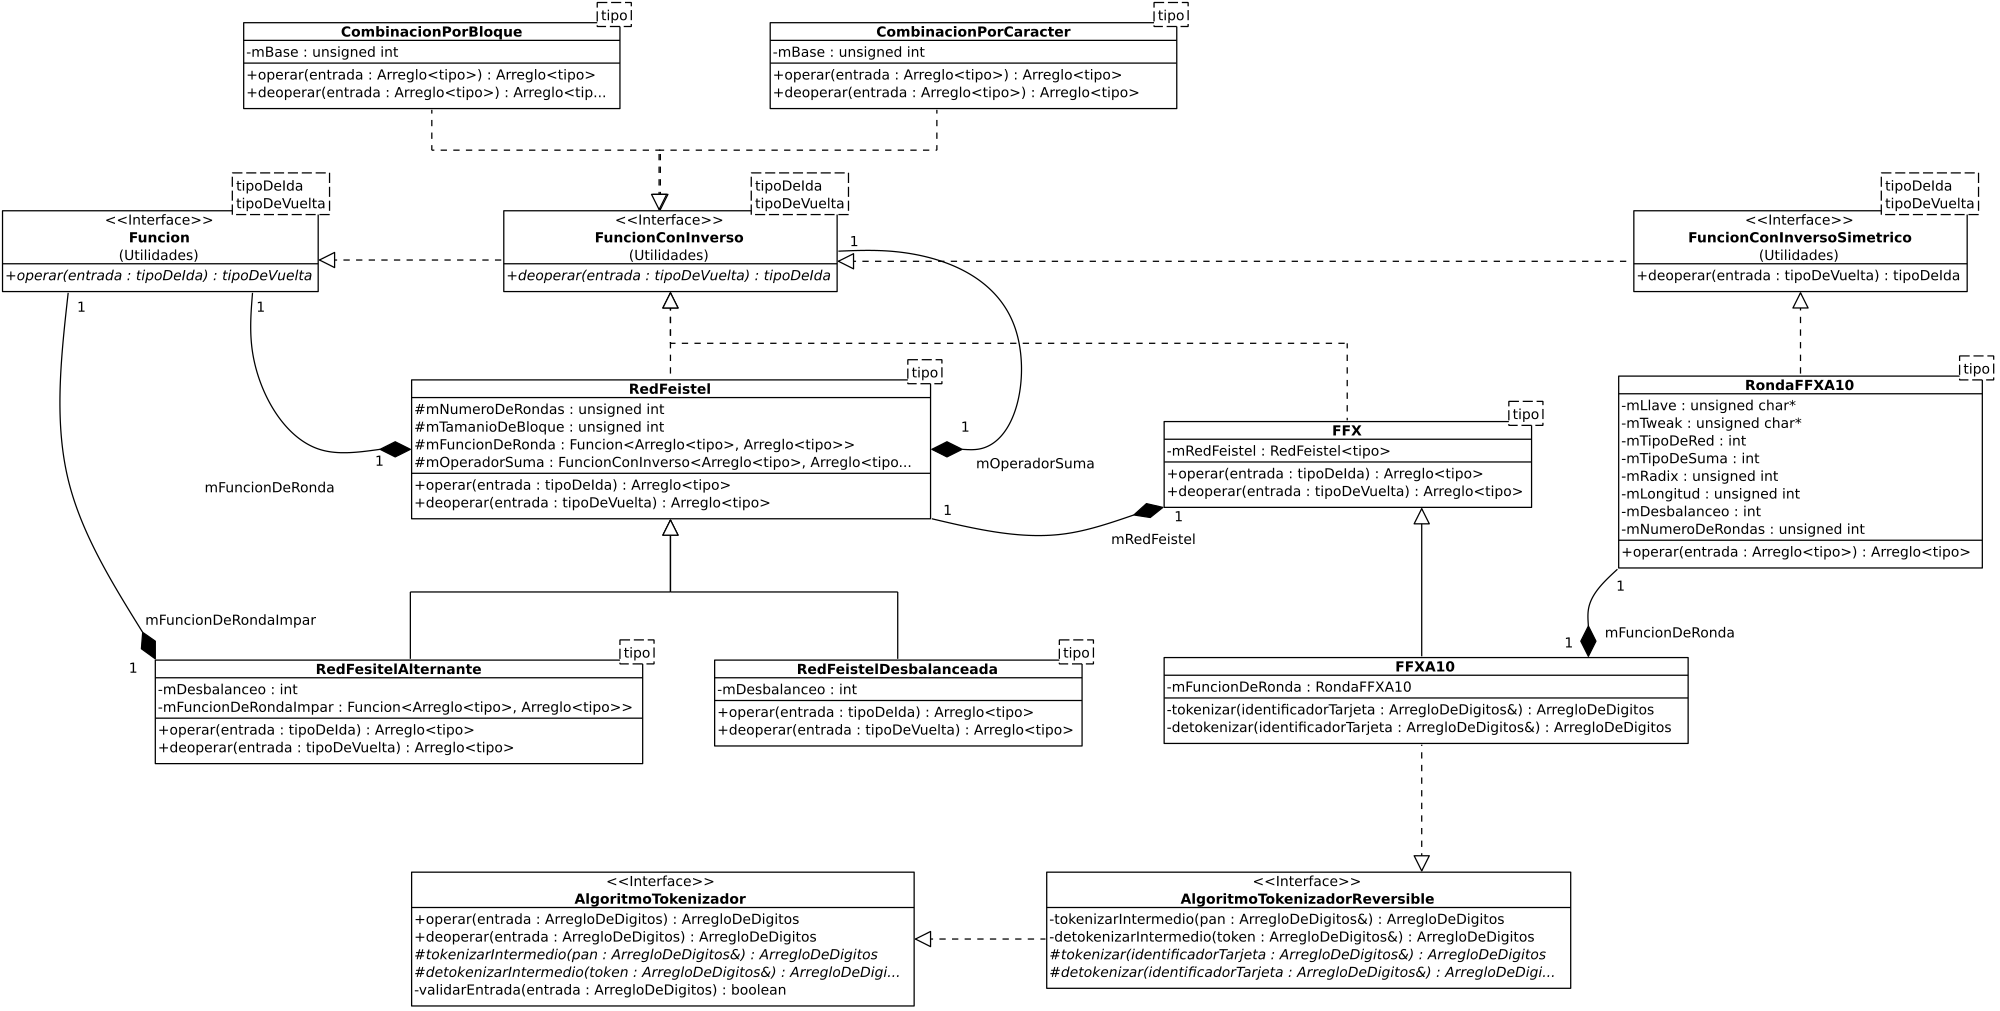
\includegraphics[width=1.0\linewidth]{diagramas/ffx.png}
    \caption{Diagrama de clases de módulo de FFX.}
    \label{clases_ffx}
  \end{center}
\end{sidewaysfigure}


\subsubsection{Selección de tecnologías}

Las primeras decisiones tomadas con respecto a la implementación y al diseño
fueron sobre el paradigma de programación y el lenguaje a utilizar. Para
tomar estas decisiones se tomaron en cuenta varias consideraciones: primero,
el paradigma orientado a objetos ofrece considerables ventajas con respecto
a la programación estructurada, por lo que, dentro de lo posible, se buscaría
un lenguaje con soporte a este paradigma; segudo, las implementaciones
criptográficas tienen altos requerimientos de rendimiento, por lo que, de los
posibles lenguajes, necesitabamos elegir uno que, si bien no el más rápido,
sí se encontrara entre los de mayor velocidad.

A lo largo de nuestra carrera hemos tenido contacto con bastantes lenguajes que,
si bien no dominamos, sí poseemos una base firme como para ser usada: C, C++,
Java, Python, Javascript y PHP. Por la cuestión del rendimiento, todos los
lenguajes interpretados (Python, Javascript, PHP) quedaron fuera de
consideración; la decisión (dentro de los lenguajes con soporte al paradigma
orientado a objetos) quedó entre Java y C++: Java (aún en las últimas versiones,
en donde se han hecho considerables progresos) es mucho más lento que C++,
dado que el trabajo de la máquina virtual en tiempo de ejecución es bastante
considerable; por lo tanto, si de un lenguaje orientado a objetos se trataba,
sería C++. La última decisión se dió entre C y C++: orientación a objetos contra
rendimiento. Al final se optó por la orientación a objetos: aún cuando C es
más rápido que C++, la diferencia no es tan grande, mientras que un programa
con un buen diseño orientado a objetos sí puede ser mucho más mantenible que
uno con un enfoque estructurado.

La verisón de C++ que utilizamos es C++14. Por razones de compatibilidad con
algunas de nuestras dependencias (en particular, el conector de la base de
datos) no pudimos utilizar la última versión al momento, C++17.

El gestor de base de datos que más hemos utilizado en la carrera es MySQL,
por lo que es el que seleccionamos para el programa tokenizador; en realidad,
se trata de una bifurcación de MySQL: MariaDB, cuyo uso ha sido ampliamente
difundido en varias distribuciones de Linux.

Otra decisión importante a tomar antes de hacer las implementaciones de los
algoritmos tokenizadores fue la librería de funciones criptográficas que
utilizaríamos. De todas las posibles librerías que están validadas
por el \gls{gl:nist} y que cuentan con una licencia para el uso público, al
final hicimos pruebas con dos: Openssl y Crypto++. Openssl está escrita
en C y cuenta con un historial que le da mucha reputación (es la librería
que utiliza Opengpg y Openssh). Cryptopp cuenta con una extensa red de
colaboradores, implementa una gran cantidad de algoritmos y está escrita sólo
en C++. De ambas, la que encontramos más fácil de usar fue Crypto++, por lo que
es la que utilizamos en nuestras implementaciones.
